\documentclass[a4paper]{article}
\usepackage[utf8]{inputenc}
\usepackage[russian,english]{babel}
\usepackage[T2A]{fontenc}
\usepackage[left=10mm, top=20mm, right=18mm, bottom=15mm, footskip=10mm]{geometry}
\usepackage{indentfirst}
\usepackage{amsmath,amssymb}
\usepackage{mathastext} 
\usepackage[italicdiff]{physics}
\usepackage{graphicx}
\usepackage{caption}
\usepackage{float}
\usepackage{caption}
\renewcommand{\thefootnote}{\fnsymbol{footnote}}
\usepackage{tablefootnote}
\usepackage{footmisc}
\usepackage{textcomp}
\usepackage{multicol}
\usepackage{multirow}
\usepackage[parfill]{parskip}
\usepackage{makecell}
\usepackage{array}  
\usepackage{siunitx}
\usepackage{booktabs}
\sisetup{
    exponent-product = \cdot,
    per-mode = symbol,
    separate-uncertainty = true,
    uncertainty-separator = \,
}
\renewcommand\cellalign{cc} 
\renewcommand\cellgape{\Gape[2pt]} 
\usepackage[utf8]{inputenc}\newcommand{\approxtext}[1]{\ensuremath{\stackrel{\text{#1}}{\approx}}}
\usepackage[colorlinks=true, urlcolor=blue, linkcolor=blue, citecolor=blue]{hyperref}
\graphicspath{{images/}}
\DeclareGraphicsExtensions{.pdf,.png,.jpg}
\usepackage{wrapfig}
\captionsetup{labelformat=empty}
\usepackage{caption}
\captionsetup[figure]{name=Рисунок}
\captionsetup[table]{name=Таблица}
%\usepackage{newtxtext,newtxmath} 
\title{\textbf{Отчет о выполнении лабораторной работы 4.1.1-4.1.2} \\[0.5em] \large\itshape Геометрическая оптика}
\date{}
\author{Котляров Михаил, Б01-402}

\begin{document}

\maketitle
	
\section{Введение}

\subsubsection*{Цель работы:} изучение свойств оптических систем: определение фокусных расстояний линз, определение фокусных расстояний и положения главной и фокальной плоскостей сложной оптической системы, изучение аббераций оптических систем.


\subsubsection*{Оборудование и инструментальные погрешности}

\textbf{оптическая скамья с набором рейтеров},\\
\textbf{линейка}: погрешность 1 мм.\\
\textbf{осветитель с ирисовой диафрагмой},\\
\textbf{зрительная труба Ruber-x32},\\
\textbf{кольцевые диафргамы},\\
\textbf{Положительные линзы}: GCL-010173N (3.1) f = 75 мм, GCL-010119N (3.2) f = 150 мм, GCL-010176N (3.3) f = 200 мм, GCL-010177N (3.4) f = 300 мм, линза 3.6 неизвестной маркировки,\\
\textbf{Отрицательная линза}: 3.5, маркировка неизвестна,


\subsection*{Описание экспериментальной установки}

Экспериментальная установка представляет собой оптическую скамью с набором сменных элементов. Основные компоненты:

\begin{itemize}
    \item \textbf{Источник света (И)} --- осветитель с прозрачным транспарантом (сетка с известным размером ячеек $y_0$);
    \item \textbf{Набор линз} --- собирающие (положительные) и рассеивающие (отрицательные) линзы с различными фокусными расстояниями, закреплённые в поворотных держателях;
    \item \textbf{Подзорная труба (П)} --- вспомогательный зрительный прибор, настроенный на «бесконечность», с окулярной риской для угловых измерений;
    \item \textbf{Экран (Э)} --- матовая поверхность для наблюдения действительных изображений;
    \item \textbf{Диафрагмы (Д)} --- ирисовые и круглые диафрагмы ($\varnothing \approx 5$~мм) для выделения параксиальных лучей;
    \item \textbf{Измерительная шкала} --- линейка на оптической скамье с точностью отсчёта 1~мм.
\end{itemize}

Все элементы центрируются относительно оптической оси с помощью регулировочных винтов (вертикальное смещение, поперечное смещение, поворот вокруг вертикальной оси). Положения главных плоскостей линз отмечены рисками на оправе.

Для защиты оптических поверхностей от загрязнений не допускается касание стеклянных элементов пальцами. При наблюдении изображений глазом яркость источника уменьшается до минимума.

\section{Выполнение работы}

\subsection{I. Определение фокусных расстояний линз с помощью подзорной трубы}

\begin{itemize}
    \item \textbf{Настройка подзорной трубы.} Настроим подзорную трубу на «бесконечность». Для этого, глядя в окуляр, добьёмся чёткого изображения перекрестия и рисок, а затем наведём трубу на удалённый предмет и фокусировочным винтом получим резкое изображение.

    \item \textbf{Измерение фокусных расстояний собирающих линз.} Расположим собирающую линзу~$Л$ перед источником света~$И$ на расстоянии, приблизительно равном фокусному. За линзой разместим подзорную трубу~$П$ (рис.~\ref{fig:telescope_method}). Глядя в трубу и слегка перемещая линзу, добьёмся чёткого изображения транспаранта источника. Измерим расстояние~$f$ от источника до линзы (положение главных плоскостей отмечено рисками на оправе). Для повышения чёткости наденем на оправу линзы диафрагму~$Д$ диаметром $\approx 5$~мм. Систематическая погрешность измерения составляет $\sigma_\text{сист} = $ 2 мм, поскольку погрешность линейки 1 мм и еще в 1 мм оценена точность прикладывания ее к источнику (так как сам источник углублен в корпус примерно на 1 мм, поэтому точно приложить нет возможности).

    \begin{figure}[h]
        \centering
        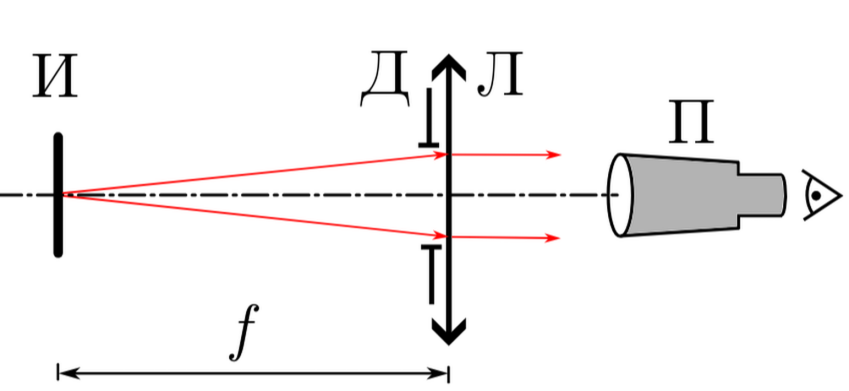
\includegraphics[width=0.5\textwidth]{Pictures/telescope_method.png}
        \caption{Рис. 1. Схема измерения фокусного расстояния с помощью подзорной трубы: И~--- источник, Л~--- линза, Д~--- диафрагма, П~--- подзорная труба}
        \label{fig:telescope_method}
    \end{figure}

    \item \textbf{Проверка тонкости линзы.} Развернём линзу обратной стороной к источнику (используя винт поворотного крепления) и повторим измерение~$f$. Сравним полученные значения для прямой и обратной ориентации линзы.

\begin{table}[h!]
\centering
\begin{tabular}{|c|c|c|}
\hline
№ & $F_1$, мм & $F_2$, мм \\
\hline
1 & 77 & 72 \\ \hline
2 & 76 & 72 \\ \hline
3 & 77 & 72 \\ \hline
Среднее & $76{,}7 \pm 0{,}6$ & $72{,}0 \pm 0{,}0$ \\
\hline
\end{tabular}
\caption{Таблица 1. Серия измерений фокусного расстояния линзы GCL-010173N}
\label{tab:lens1_detailed}
\end{table}

Исходя из измерений случайная погрешность составила $\sigma_\text{случ} = 0,33$ мм. Таким образом далее полную погрешность измерений с помощью линейки мы будем считать $\sigma = \sqrt{ \left(\sigma_\text{случ} \right )^2 + \left(\sigma_\text{сист} \right )^2} = 2,03$ мм.

\begin{table}[h!]
\centering
\begin{tabular}{|l|c|c|c|c|c|}
\hline
Линза & $F_1$, мм & $F_2$, мм & $F_{\text{таб}}$, мм & $\Delta F$, мм & $\delta$, \% \\
\hline
GCL-010173N & $76{,}7$ & $72{,}0 $ & 75 & 4,7 & 6,3 \\ \hline
GCL-010119N & 153 & 149 & 150 & 4 & 2,7 \\ \hline
GCL-010176N & 202 & 205 & 200 & 3 & 1,5 \\ \hline
GCL-010177N & 304 & 308 & 300 & 4 & 1,3 \\
\hline
\end{tabular}
\caption{Таблица 2. Сводные результаты измерения фокусных расстояний линз}
\label{tab:all_lenses}
\end{table}


    \item \textbf{Измерение фокусного расстояния рассеивающей линзы.} Соберём схему согласно рис.~\ref{fig:diverging_lens}. Разместим положительную линзу~$\text{Л}_1$ с наибольшим фокусным расстоянием перед источником и получим на экране~$Э$ чёткое уменьшенное изображение. Измерим расстояние~$b_1$ от линзы до экрана. Поместим исследуемую отрицательную линзу~$\text{Л}_p$ между $\text{Л}_1$ и экраном. Уберём экран и за отрицательной линзой разместим подзорную трубу. Перемещая $\text{Л}_p$, получим сфокусированное изображение в трубу. Измерим расстояние~$l$ между линзами и вычислим фокусное расстояние рассеивающей линзы по формуле $f_\text{р} = -(b_1 - l)$.

\clearpage
    \begin{figure}[h]
        \centering
        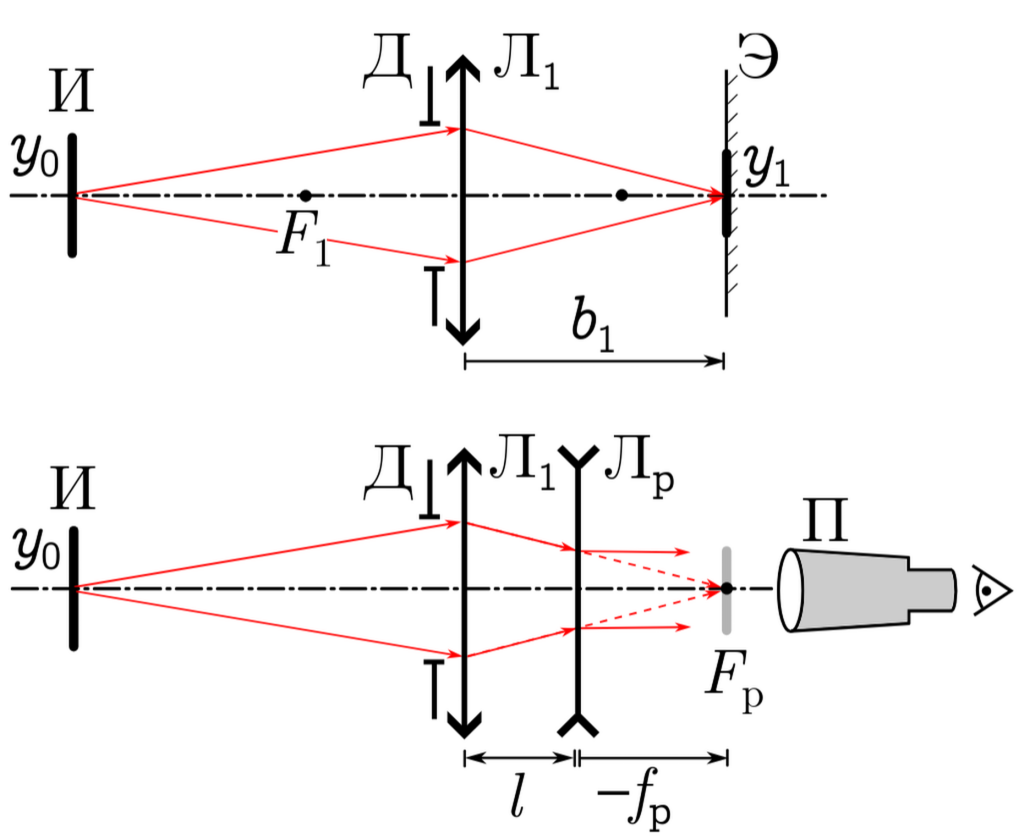
\includegraphics[width=0.5\textwidth]{Pictures/diverging_lens.png}
        \caption{Рис. 2. Схема измерения фокусного расстояния рассеивающей линзы: И~--- источник, Л$_1$~--- положительная линза, Л$_\text{р}$~--- рассеивающая линза, Э~--- экран, П~--- подзорная труба}
        \label{fig:diverging_lens}
    \end{figure}
\end{itemize}

\begin{table}[h!]
\centering
\begin{tabular}{|c|c|c|c|c|}
\hline
$b_1$, мм & $L_1$, мм & $L_2$, мм & $F_{\text{расс}}$, мм & $\Delta F$, мм \\
\hline
513 & 406 & 417 & $-107$ / $-96$ & 11 \\
\hline
\end{tabular}
\caption{Таблица 3. Измерение фокусного расстояния рассеивающей линзы}
\label{tab:diverging}
\end{table}

\subsection{II. Измерение фокусных расстояний по формуле тонкой линзы и методом Бесселя}

\begin{itemize}
    \item \textbf{Подготовка схемы.} Выберем положительную линзу с известным (приближённо) значением фокусного расстояния~$f$. Поместим экран на расстоянии $L > L_{\min} = 4f$ от предмета. Измерим величину~$L$ по шкале оптической скамьи.

    \item \textbf{Поиск положений линзы.} Поместим исследуемую линзу между источником и экраном (рис.~\ref{fig:bessel_method}). Найдём два положения линзы, при которых на экране возникают чёткие действительные изображения --- увеличенное и уменьшенное. Измерим соответствующие расстояния~$a_1$ и~$a_2$ от источника до линзы. Тщательно измерим смещение между этими положениями $l = a_2 - a_1$.

    \begin{figure}[h]
        \centering
        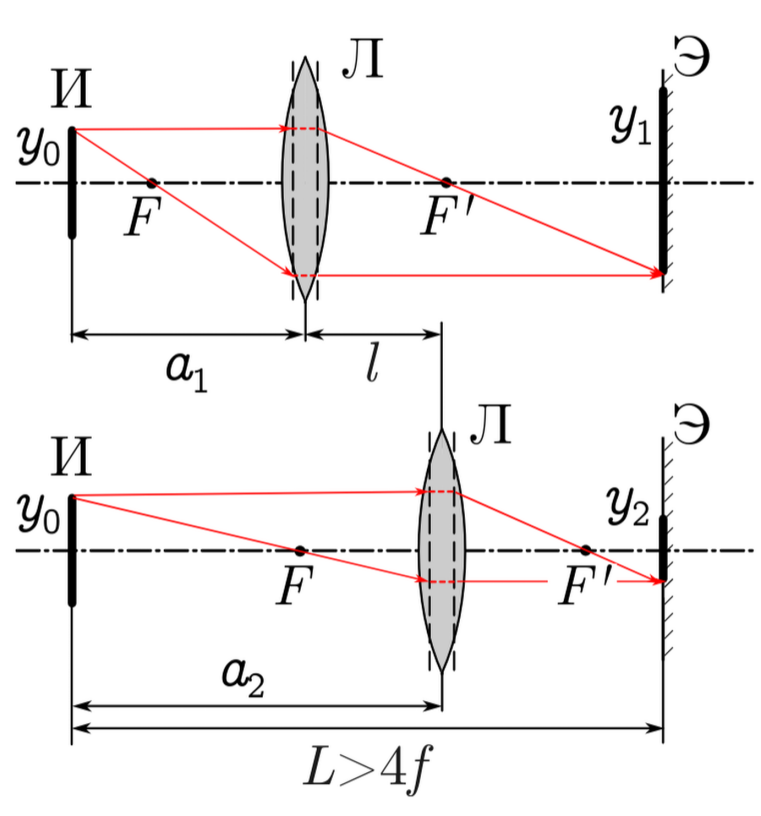
\includegraphics[width=0.374\textwidth]{Pictures/bessel_method.png}
        \caption{Рис. 3. Схема измерения методом Бесселя: И~--- источник, Л~--- линза, Э~--- экран, $L$~--- расстояние источник--экран, $l$~--- смещение линзы}
        \label{fig:bessel_method}
    \end{figure}

    \item \textbf{Вычисление фокусного расстояния.} Рассчитаем фокусное расстояние двумя способами:
    \begin{enumerate}
        \item по формуле тонкой линзы: $\displaystyle \frac{1}{f} = \frac{1}{a} + \frac{1}{L - a}$;
        \item по приближённой формуле Бесселя: $\displaystyle f \approx \frac{L^2 - l^2}{4L}$.
    \end{enumerate}

    \item \textbf{Проверка симметрии линзы.} Развернём линзу обратной стороной и повторим измерения. Сравним полученные значения фокусных расстояний для двух ориентаций линзы.
\end{itemize}

\begin{table}[h!]
\centering


\begin{tabular}{|c|c|c|c|c|}
\hline
\multirow{3}{*}{\shortstack{Ориен-\\тация}} & \multirow{3}{*}{\shortstack{Положение\\линзы}} & \multicolumn{2}{c|}{Метод тонкой линзы} & \multicolumn{1}{c|}{Метод Бесселя} \\
\cline{3-5}
& & \multicolumn{2}{c|}{$f = \frac{a(L-a)}{L}$} & \multicolumn{1}{c|}{$f = \frac{L^2-l^2}{4L}$} \\
\cline{3-5}
& & $a$, мм & $f \pm \Delta f$, мм & $\langle f \rangle \pm \Delta f$, мм \\
\hline
\multirow{2}{*}{1 (прямая)} 
& Уменьшенное ($a_1$) & 747 & $150{,}20 \pm 1{,}77$ & \multirow{2}{*}{$148{,}70 \pm 2{,}38$} \\ \cline{2-4}
& Увеличенное ($a_2$) & 183 & $147{,}18 \pm 1{,}24$ & \\
\hline
\multirow{2}{*}{2 (обратная)} 
& Уменьшенное ($a_1$) & 745 & $151{,}39 \pm 1{,}76$ & \multirow{2}{*}{$150{,}80 \pm 2{,}37$} \\ \cline{2-4}
& Увеличенное ($a_2$) & 188 & $150{,}20 \pm 1{,}21$ & \\
\hline
\multicolumn{2}{|c|}{\textbf{Итоговое среднее}} & \multicolumn{2}{c|}{$\mathbf{149{,}74 \pm 1{,}50}$} & \multicolumn{1}{c|}{$\mathbf{149{,}75 \pm 2{,}38}$} \\
\hline
\end{tabular}
\caption{Таблица 6. Сравнение методов измерения фокусного расстояния ($L=935$~мм)}
\label{tab:bessel_vs_thin}
\end{table}

\subsection{IV. Сборка и изучение подзорных труб Кеплера и Галилея}

\begin{itemize}
    \item \textbf{Подготовка коллиматора.} Выберем из набора три линзы: для объектива \\(3.2, GCL-010119N,~$f_{\text{об}} = 150$ мм), окуляра (3.1, GCL-010173N, ~$f_{\text{ок}} = 75$ мм) \\ (расчётное увеличение $\gamma = |f_{\text{об}}/f_{\text{ок}}| = 2 $) и для коллиматора (3.4, GCL-010177N,  ~$f_{\text{кол}}  = 300$ мм) (наиболее длиннофокусная). Установим коллиматорную линзу перед источником так, чтобы транспарант оказался строго в фокусе линзы. Таким образом создадим расположенный на «бесконечности» предмет с угловым размером $\alpha_0 = y_0/f_{\text{кол}}$.

    \item \textbf{Фиксация исходной картины.} Сфотографируем на камеру смартфона картину, наблюдаемую в окуляр вспомогательной подзорной трубы, направленной на коллиматор (рис. 4). По фотографии определим угловой размер ячейки сетки~$\alpha_0$ (через число ячеек, укладывающихся на длине окулярной риски).

\begin{figure}[h]
        \centering
        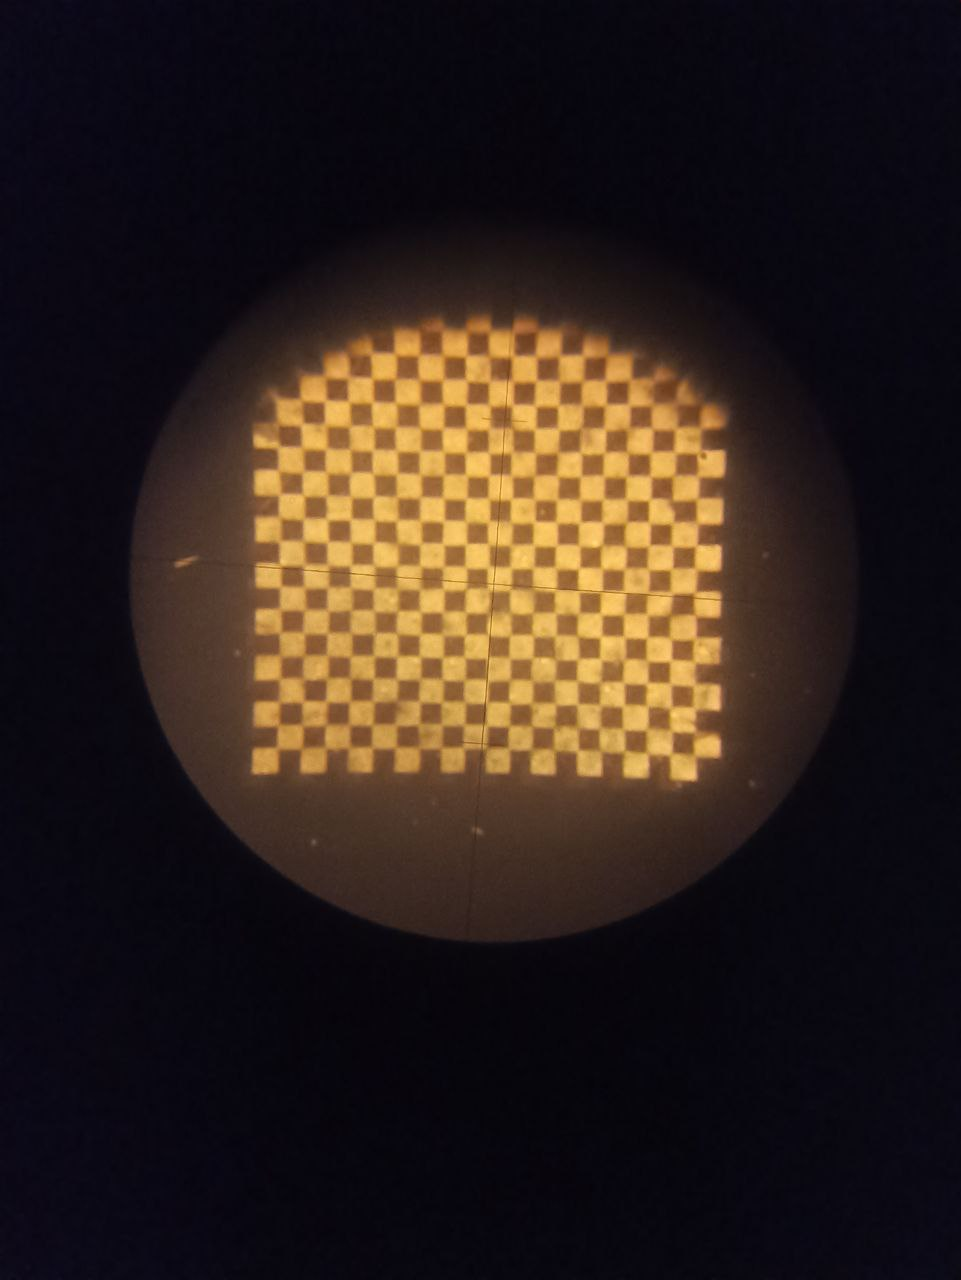
\includegraphics[width=0.4\textwidth]{Pictures/without_telescope.jpg}
        \caption{Фото 1. Изображение в трубе без телескопа}
    \end{figure}
\clearpage
    \begin{figure}[h]
        \centering
        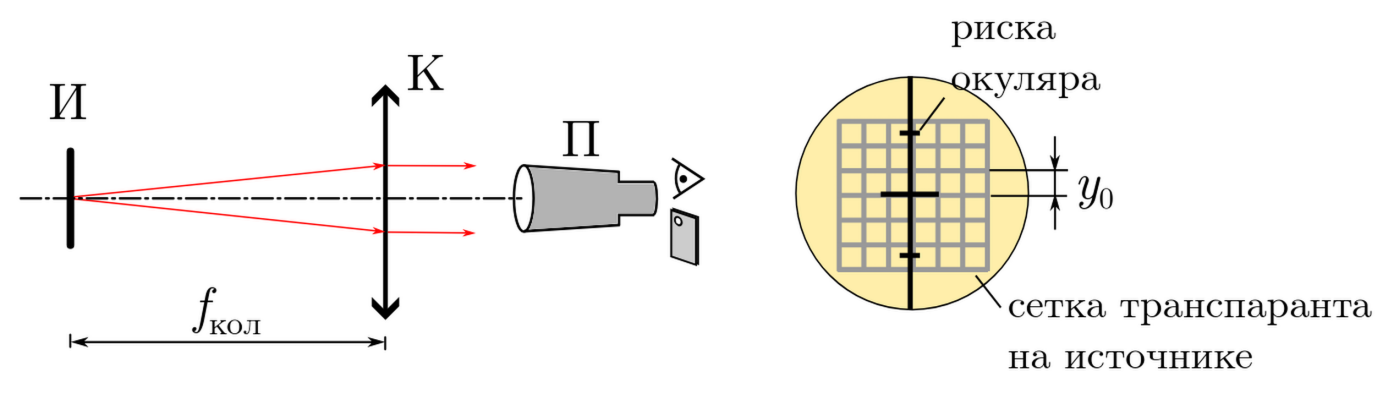
\includegraphics[width=0.7\textwidth]{Pictures/collimator_setup.png}
        \caption{Рис. 4. Схема настройки коллиматора: И~--- источник, К~--- коллиматор, П~--- вспомогательная подзорная труба}
        \label{fig:collimator_setup}
    \end{figure}

    \item \textbf{Сборка телескопа.} Соберём модель телескопа Кеплера (или Галилея). Объектив (линза с наибольшим фокусным расстоянием) расположим сразу за коллиматором. Окуляр установим на расстоянии $f_{\text{об}} + f_{\text{ок}}$ от объектива (для трубы Галилея $f_{\text{ок}} < 0$). Схема представлена на рис. 5.


    \begin{figure}[h]
        \centering
        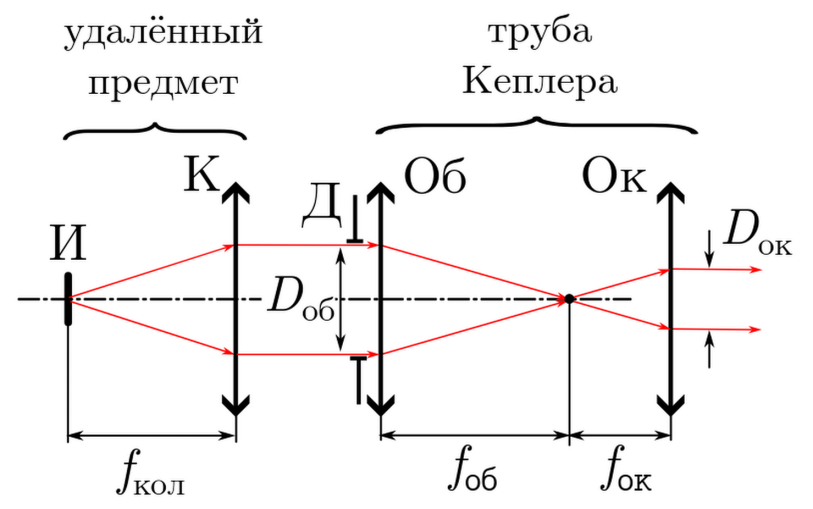
\includegraphics[width=0.7\textwidth]{Pictures/telescope_assembly.png}
        \caption{Рис. 5. Схема телескопа: К~--- коллиматор, Об~--- объектив, Ок~--- окуляр, Д~--- диафрагма}
        \label{fig:telescope_assembly}
    \end{figure}


    \item \textbf{Измерение углового увеличения.} Установим вспомогательную подзорную трубу непосредственно за окуляром собранного телескопа. Сфотографируем картину, наблюдаемую через телескоп. По фотографии определим видимый угловой размер ячейки~$\alpha$. Рассчитаем экспериментальное увеличение $\gamma_{\text{эксп}} = \alpha/\alpha_0$ и сравним его с теоретическим $\gamma_{\text{теор}} = |f_{\text{об}}/f_{\text{ок}}|$.
\clearpage
\begin{figure}[h]
        \centering
        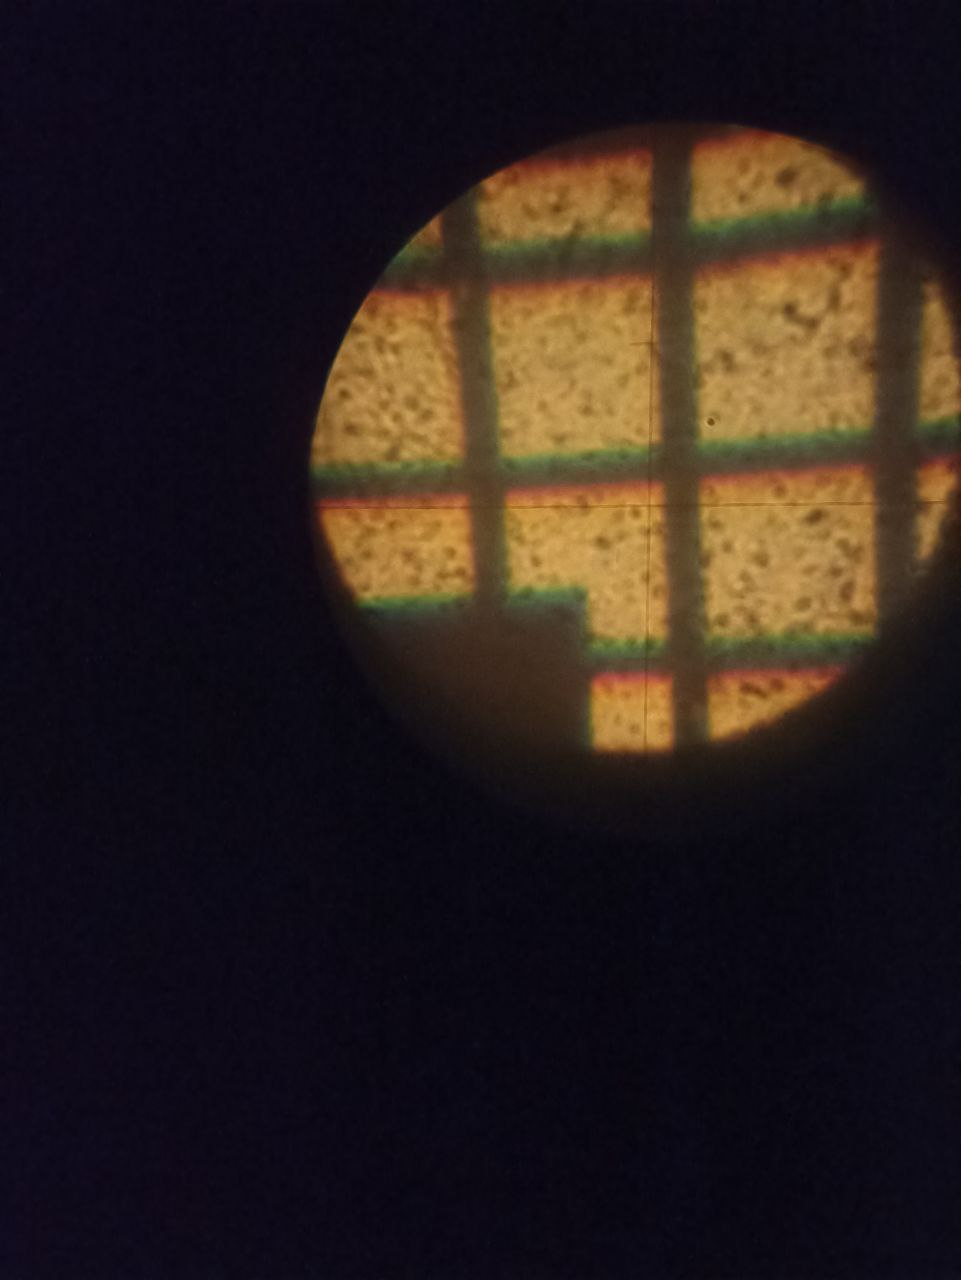
\includegraphics[width=0.4\textwidth]{Pictures/with_telescope.jpg}
        \caption{Фото 2. Изображение в трубе с телескопом}
    \end{figure}

\begin{table}[h!]
\centering
\caption{Таблица 7. Измерение углового увеличения телескопа}
\label{tab:telescope_mag}
\begin{tabular}{|l|c|c|c|c|c|c|}
\hline
\multirow{2}{*}{\shortstack{Режим\\наблюдения}} & \multicolumn{3}{c|}{Измерения по фотографии} & \multirow{2}{*}{\shortstack{Масштаб\\съёмки\\$S$, см/мм}} & \multirow{2}{*}{\shortstack{Реальный размер\\в пределах риски\\$Y$, мм}} & \multirow{2}{*}{\shortstack{Увеличение\\$\gamma$}} \\
\cline{2-4}
& \shortstack{Кол-во\\ячеек $N$} & \shortstack{Длина\\отрезка\\$L_{\text{фото}}$, см} & \shortstack{Размер\\ячейки\\$y_{\text{реал}}$, мм} & & & \\
\hline
Без телескопа & 16 & 6,0 & 0,2 & 1,875 & 1,440 & \multirow{2}{*}{$1,52 \pm 0,09$} \\ \cline{1-6}
С телескопом & 2,5\footnotemark[1]  & 6,6 & 1,2 & 2,750 & 0,945 & \\
\hline
\end{tabular}
\end{table}
\footnotetext[1]{Примечание: В подсчёт включено 2 полные ячейки и учтена толщина линий сетки (эквивалентно 0,5 ячейки), так как реальный шаг сетки составляет 1,2 мм (1 мм клетка + 0,2 мм линия).}
    \item \textbf{Анализ расхождений.} Обсудим возможные причины расхождения теории и измерений (неточная установка межлинзового расстояния, неидеальная коллимация, аберрации, погрешность определения границ ячеек на фотографии).
\end{itemize}

\section{Результаты и обсуждения}

\subsection{I. Определение фокусных расстояний линз с помощью подзорной трубы}

В ходе выполнения первого раздела работы были измерены фокусные расстояния четырёх собирающих линз и одной рассеивающей линзы методом подзорной трубы. Результаты сведены в таблицы~\ref{tab:lens1_detailed}--\ref{tab:diverging}.

\textbf{Собирающие линзы.} Для всех линз были проведены измерения при двух ориентациях (прямой и обратной) для проверки условия «тонкости». Как видно из таблицы~\ref{tab:all_lenses}, разница $\Delta F = |F_1 - F_2|$ составляет от 3 до 4,7~мм, что соответствует относительному отклонению $\delta$ от 1,3\% до 6,3\%. Наибольшее отклонение наблюдается у короткофокусной линзы GCL-010173N (6,3\%), что объясняется тем, что для плоско-выпуклых линз главные плоскости смещены относительно центра линзы на величину $\delta \approx T \cdot (n-1)/n$, где $T$ — толщина линзы, $n$ — показатель преломления стекла. Для длиннофокусных линз (GCL-010176N, GCL-010177N) отклонение не превышает 1,5\%, что позволяет считать их «тонкими» в рамках данной работы.

Сравнение с табличными значениями показывает хорошее согласие: все измеренные фокусные расстояния отличаются от номиналов не более чем на 3\%, что укладывается в пределы полной погрешности измерений $\sigma = 2{,}03$~мм.

\textbf{Рассеивающая линза.} Фокусное расстояние рассеивающей линзы определялось вспомогательным методом с использованием положительной линзы (табл.~\ref{tab:diverging}). Полученные значения $f_\text{р} = -107$~мм и $-96$~мм для двух ориентаций отличаются на 11~мм. Такое значительное расхождение объясняется методом измерения: используется мнимый предмет, что повышает чувствительность к погрешностям центровки и определения положения главных плоскостей. Табличное значение для рассеивающей линзы в описании работы не указано, поэтому оценить точность можно только по воспроизводимости измерений.

\subsection{II. Измерение фокусных расстояний по формуле тонкой линзы и методом Бесселя}

Для одной из собирающих линз (GCL-010119N, номинал $F_\text{таб} = 150$~мм) были проведены измерения двумя независимыми методами. Результаты представлены в таблице~\ref{tab:bessel_vs_thin}.

\textbf{Сравнение методов.} Средние значения фокусного расстояния, полученные обеими, практически идентичны:
\begin{itemize}
    \item Формула тонкой линзы: $\langle f \rangle = 149{,}74 \pm 1{,}50$~мм;
    \item Приближенная формула Бесселя: $\langle f \rangle = 149{,}75 \pm 2{,}38$~мм.
\end{itemize}
Расхождение между методами составляет всего 0,01~мм (0,007\%), что значительно меньше погрешностей измерений. Это подтверждает корректность метода и эквивалентность формул.

\textbf{Сравнение с теорией.} Номинальное значение фокусного расстояния линзы составляет 150~мм. Оба экспериментальных результата отличаются от табличного значения на 0,25~мм (0,17\%), что является отличным результатом. Погрешность метода Бесселя оказалась несколько выше (2,38~мм против 1,50~мм), что объясняется тем, что в формулу $f = (L^2 - l^2)/(4L)$ входят оба расстояния $a_1$ и $a_2$, что усиливает влияние погрешности измерения смещения $l$.

\textbf{Преимущества метода Бесселя.} Главное преимущество метода Бесселя заключается в том, что он не требует знания положения главных плоскостей линзы — измеряется только смещение $l$ между двумя положениями. Это делает метод менее чувствительным к систематическим ошибкам, связанным с неопределённостью положения оптического центра линзы.

\subsection{IV. Сборка и изучение подзорных труб Кеплера и Галилея}

Была собрана модель телескопа Кеплера с использованием линз GCL-010119N ($f_\text{об} = 150$~мм) в качестве объектива и GCL-010173N ($f_\text{ок} = 75$~мм) в качестве окуляра. Результаты измерения углового увеличения представлены в таблице~\ref{tab:telescope_mag}.

\textbf{Экспериментальное увеличение.} По результатам обработки фотографий (табл.~\ref{tab:telescope_mag}) получено экспериментальное значение увеличения:
$$ \gamma_\text{эксп} = 1{,}52 \pm 0{,}09 $$

\textbf{Теоретическое увеличение.} Расчётное значение увеличения телескопа:
$$ \gamma_\text{теор} = \left|\frac{f_\text{об}}{f_\text{ок}}\right| = \frac{150}{75} = 2{,}0 $$

\textbf{Анализ расхождений.} Экспериментальное значение отличается от теоретического на 24\%, что превышает погрешность измерений ($\approx 6\%$). Это указывает на наличие систематических ошибок. Основные причины расхождения:

\begin{enumerate}
    \item \textbf{Неточная установка межлинзового расстояния.} Формула $\gamma = f_\text{об}/f_\text{ок}$ справедлива только при условии, что расстояние между объективом и окуляром строго равно $d = f_\text{об} + f_\text{ок}$. В лабораторной установке сложно выставить это расстояние с точностью до миллиметра из-за люфта креплений и неопределённости положения главных плоскостей.
    
    \item \textbf{Неидеальная коллимация.} Коллиматор создаёт не строго параллельный пучок, а слегка расходящийся, так как источник света имеет конечные размеры и может быть неточно установлен в фокусе коллиматорной линзы. Это эквивалентно наблюдению предмета с конечного расстояния, где формула для увеличения даёт завышенное значение.
    
    \item \textbf{Погрешность фотометрических измерений.} Определение границ ячеек сетки на фотографии затруднено из-за дифракционных эффектов, ограниченной резкости изображения и возможного параллакса камеры смартфона при съёмке.
    
    \item \textbf{Аберрации линз.} Сферические и хроматические аберрации используемых линз могут искажать изображение, особенно по краям поля зрения, что влияет на точность измерения угловых размеров.
\end{enumerate}

Несмотря на расхождение, полученный результат ($\gamma_\text{эксп} \approx 1{,}5$) качественно подтверждает работу телескопа: изображение действительно увеличивается, и порядок величины соответствует ожидаемому.

\section{Выводы}

В ходе выполнения лабораторной работы были решены следующие задачи:

\begin{enumerate}
    \item \textbf{Определены фокусные расстояния линз методом подзорной трубы.} Измерены фокусные расстояния четырёх собирающих линз (номиналы 75, 150, 200, 300~мм) и одной рассеивающей линзы. Все значения для собирающих линз согласуются с табличными в пределах 3\%. Проверка «тонкости» линз показала, что для длиннофокусных линз главные плоскости практически совпадают ($\delta < 1{,}5\%$), а для короткофокусных — наблюдается смещение до 6,3\%.
    
    \item \textbf{Сравнены методы измерения фокусного расстояния.} Для линзы с номиналом 150~мм проведены измерения по формуле тонкой линзы и методом Бесселя. Оба метода дали согласующиеся результаты ($149{,}74$~мм и $149{,}75$~мм соответственно), отличающиеся от теории на 0,17\%. Метод Бесселя менее чувствителен к положению главных плоскостей, но имеет несколько б$\acute{o}$льшую случайную погрешность.
    
    \item \textbf{Собрана и изучена модель телескопа Кеплера.} Экспериментальное угловое увеличение $\gamma_\text{эксп} = 1{,}52 \pm 0{,}09$ отличается от теоретического $\gamma_\text{теор} = 2{,}0$ на 24\%. Расхождение объясняется систематическими ошибками: неточной установкой межлинзового расстояния, неидеальной коллимацией и погрешностями фотометрических измерений.
    
    \item \textbf{Освоены навыки работы с оптической скамьой.} Приобретены практические навыки центрирования оптических элементов, настройки подзорной трубы на «бесконечность», получения действительных и мнимых изображений, а также оценки погрешностей оптических измерений.
\end{enumerate}

Таким образом, цели лабораторной работы достигнуты: экспериментально подтверждены основные формулы геометрической оптики, изучены методы определения фокусных расстояний линз и принципы работы оптических приборов (телескопа).

\end{document}